\documentclass{article}
\usepackage[utf8]{inputenc}
\usepackage[margin=1in,left=1.5in,includefoot]{geometry}
\usepackage{booktabs}
\usepackage{graphicx}
\usepackage{hyperref}
\usepackage{wrapfig}
\usepackage{float}
\usepackage{amsmath}
\usepackage{amssymb}
\usepackage[galician]{babel}
\usepackage{tcolorbox}
\usepackage{listings}


\newtcolorbox{clibox}{
  colback=gray!10,    % light gray background
  colframe=gray!50,   % gray border
  boxrule=0.5pt,      % border thickness
  arc=2pt,            % rounded corners
  left=6pt,
  right=6pt,
  top=6pt,
  bottom=6pt,
  fontupper=\ttfamily % monospaced font
}


% Header & Footer Stuff

\usepackage{fancyhdr}
\pagestyle{fancy}
\lhead{\emph{Visión por Computador Aplicada}}
\rhead{614G030332425}
% \fancyfoot{}
% \lfoot{Pablo Chantada Saborido \& José Romero Conde}
% \fancyfoot[R]{}

% The Main Document
\begin{document}
	\begin{center}
		\LARGE\bfseries PRÁCTICA II\\
		\small Pablo Chantada Saborido \& José Romero Conde
		\line(1,0){430}
	\end{center}
	
\vspace*{300pt}
	
\begin{figure}[H]
	\centering
	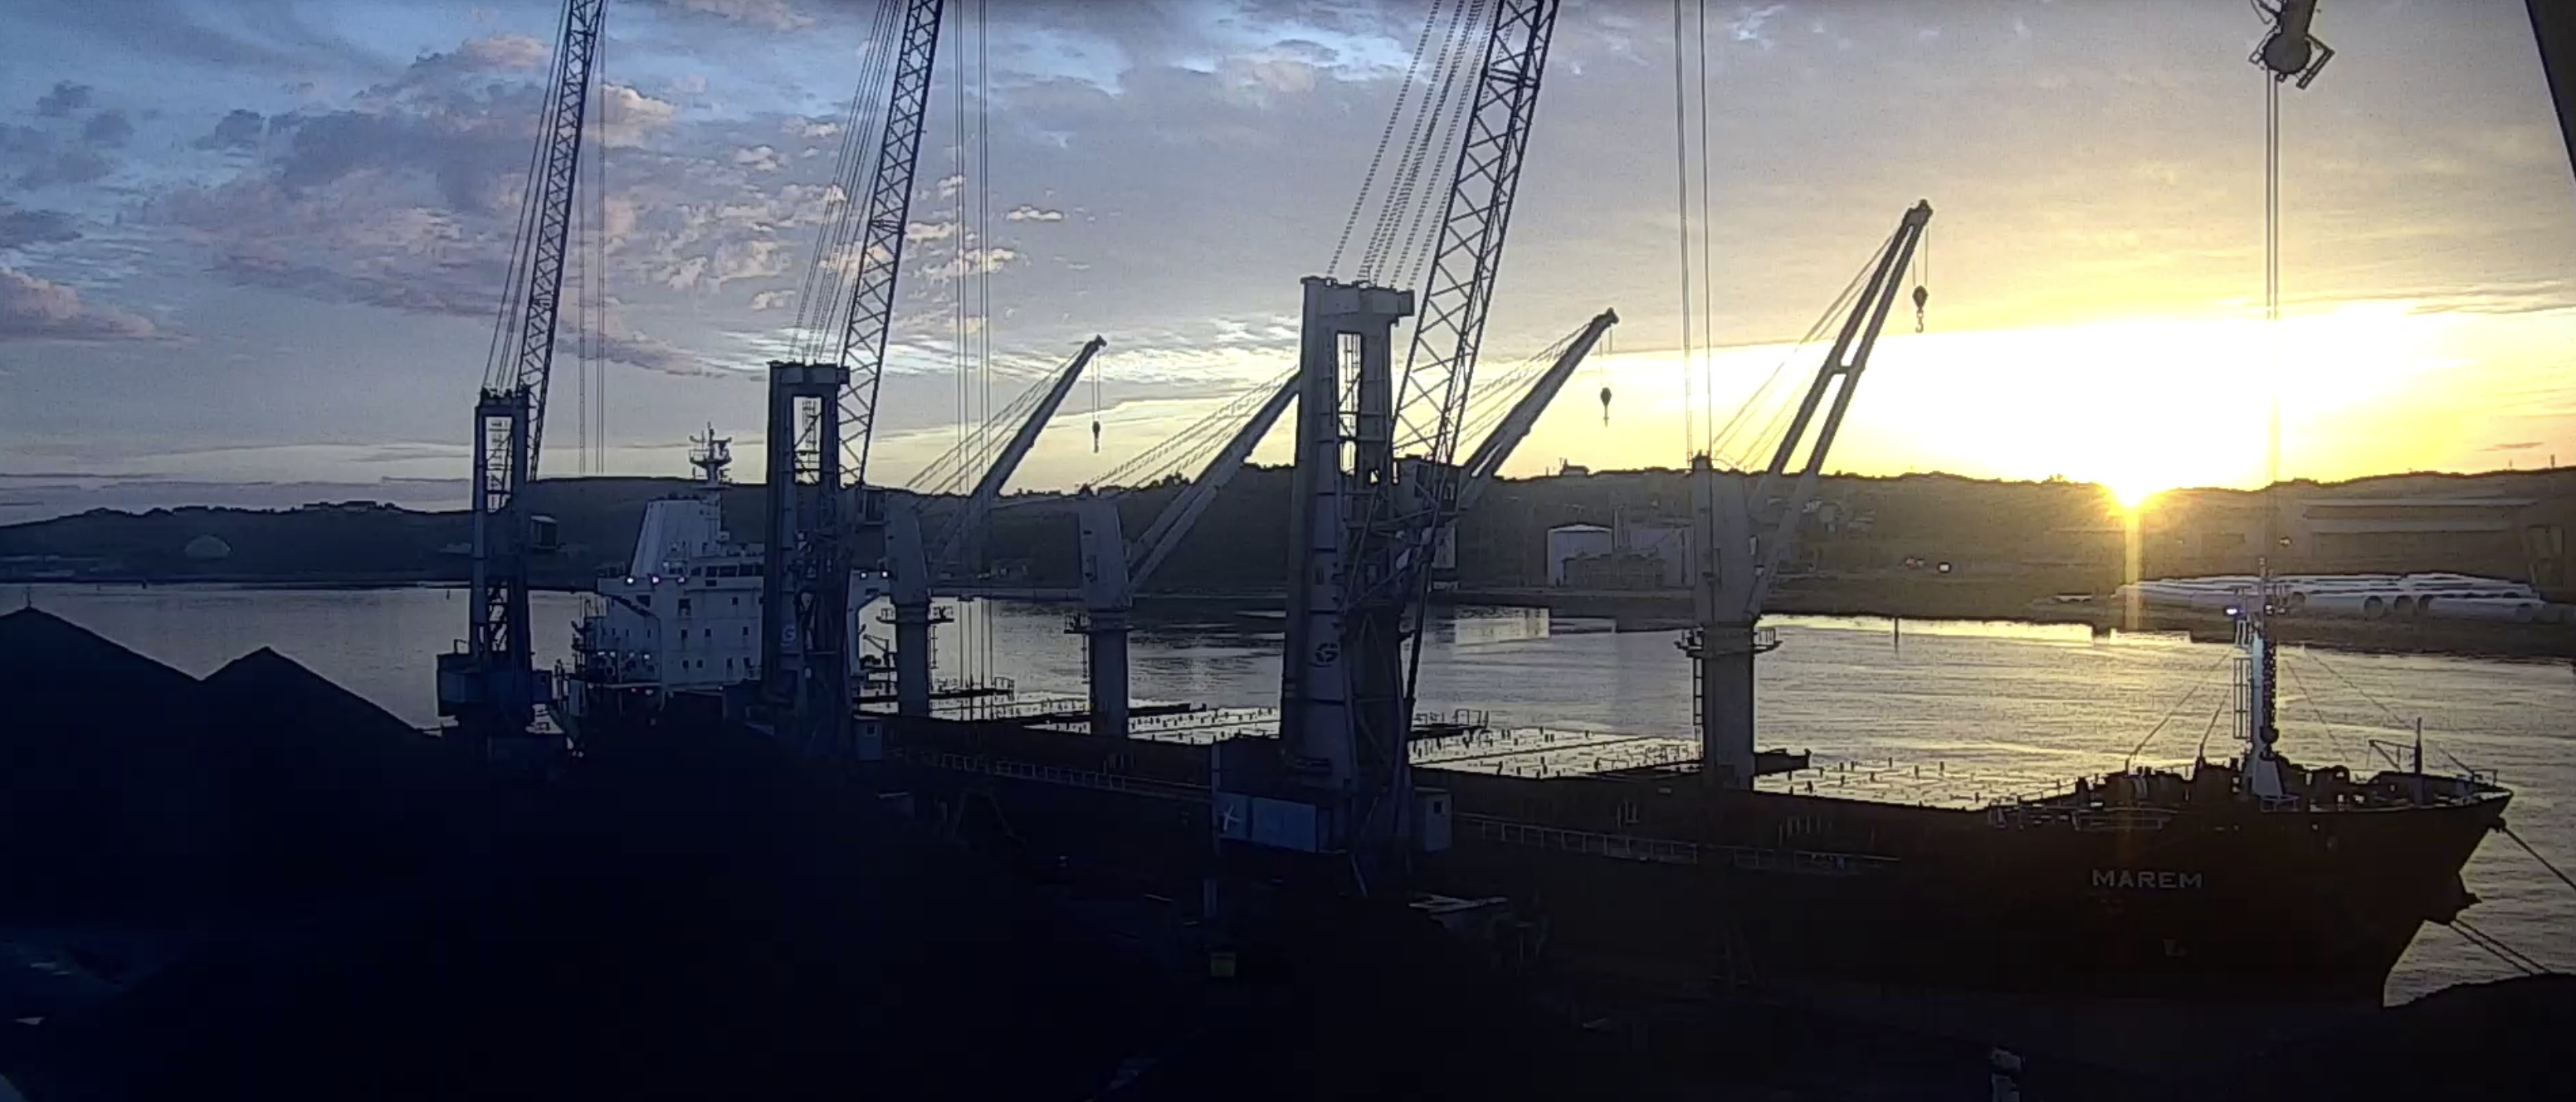
\includegraphics[width=0.7\linewidth]{figuras/portada.jpg}
	\label{fig:portada}
\end{figure}
	
\thispagestyle{empty}
	
\newpage

\tableofcontents

\newpage
	
	
\section{Introdución}

Esta práctica supuso todo un reto para nos. O Conxunto de datos foi especialmente difícil polos seguintes motivos:
\begin{itemize}
	\item \textbf{Escaseza de datos.} Acostumados a miles (MNIST) ou centos (SmartPorts) de imaxes, contar con só decenas delas supuxo unha dificultade no problema a resolver. Isto débese a que a nosa Rede ten que aprender moito de cada imaxe, e saber extrapolar o aprendido a imaxes que nunca viu. Nada sixelo.
	\item \textbf{Alta variabilidade.} Se foran poucos datos pero a realidade fosse sempre moi parecida, non habería tanto problema, a cuesstión é que de unha imaxe a outra pode haber pouco que teñan en común. As hai que a parede ocular é fina e ten unha fendidura, as hai sen fendidura mais con un gran vaso, as hai sen fendidura e con múltiples vasos... esto é para nos un problema porque o fluxo óptico \emph{existe} dun xeito distinto en cada imaxe de OCT. Polo tanto a nosa Rede debe aprender todas esas variacións con poucos exemplos.
	\item \textbf{Imperfectude da supervision.} Aínda que poderíamos ter feito un AutoEncoder para cercionarnos de unha boa representación \emph{latente}, limitámonos ó uso das máscaras para propagar a sinal de error. Ó non seren perfectas e consistentes as etiquetas (zoas dun certo nivel de gris rodeadas dun capilar, en unhas máscaras representábase o capilar e noutras non), non podemos esperar que o noso algoritmo o sexa. Ademáis, esta baseándose exclusivamente en exemplos mentras que un médico razona e delibera en base os seus coñecementos teóricos e de domino. A nosa Rede non pode facer tal cousa. 
	
\end{itemize}

Para afrotalo problema, por tanto, armamosnos con unha serie de técnicas e trucos aprendidos nesta asignatura, en Aprendizaxe Profundo e mais en Principios de Visión por Computador. Son os seguintes:
\begin{itemize}
	\item \textbf{Canles adicionais de entrada.} A Rede ten que aprender que é o fluxo óptico dende cero, sen saber que é un borde ou un círculo. Non lle pasa o mesmo ós médicos, que cando empezan na oftalmoloxía xa teñen un adestrado sistema de percepción visual. Polo tanto, para axilizar este proceso, ademáis da imaxe en Blanco e Negro $\mathcal{I}$ (un canle) decidimos acompañala dos $\phi_i(\mathcal{I})$ onde os $\phi_i$ son algoritmos de procesado de imaxen. Inicialmente escollemos Canny \cite{canny1986computational}, Sobel, Laplaciano e Frangi \cite{frangi1998multiscale}. Do último tiñamos altas esperanzas por estar tamén orientado ó ambito médico máis aínda despoís dunha considerable búsqueda de hiperparámetros decidimos descartalo para, finalmente, só quedarnos con Canny. Unha xustificación desta decisión é a imaxe de abaixo. 

\begin{figure}[H]
	\centering
	\includegraphics[width=\linewidth]{figuras/canles.png}
	\label{fig:canles}
\end{figure}


\item \textbf{Aumento de datos.} Fundamentalmente baseámonos nas suxerencias do propio artigo da UNet \cite{ronneberger2015u}  é dicir: transformacións afíns e elásticas. Cas primeiras foi realtivamente doado atopar hiperparámetros apropiados pero as segundas foi máis difícil, en cambio (ó estaren diseñadas para un contexto de segmentación médica) ofreceron moi bos resultados. Finalmente atopamos $\alpha = 500$ e $\sigma = 20$ axeitados. Ademáis, para estas dúas transformacións, ó seren realativamente \emph{agresivas}, atopamos que é millor non transformar sempre (para darlle á Rede uns poucos exemplos inalterados e aprenda deles). En concreto aplicamos cada unha delas cunha probabilidade de 0.7, polo tanto, para unha imaxen, a probabilidade de seren alterada por ambas transformacións é de $\approx 0.5$. Ademáis destas dous, aplicamos (malia observando pouca diferencia) volteos horizontais, deformacións na cor (\emph{color jitter}), variacións no enfoque e ruído gausiano aditivo. O efecto da totalidade das transformacións sobre un subconxunto das imaxes do conxunto de datos vése abaixo.

\begin{figure}[H]
	\centering
	\includegraphics[width=\linewidth]{figuras/aumento_datos.png}
	\label{fig:AD}
\end{figure}


Se ben pode parecer \emph{leve}, aumentos de datos máis agresivos non veían a luz da converxencia. Podemos dicir que a configuración de hiperparámetros do Aumento de Datos está fortemente baseada na experimentación. 

\item \textbf{PostProcesado das máscaras.} Aínda que non-diferenciables, e por tanto non contribuían á sinal de error do adestramento do algoritmo, decidimos aplicar unha serie de transformacións sobre as máscaras para acercarse máis ás reais. Pulindo detalles de xeito que, se un oftalmólogo tivera que usar o noso sistema, certas impurezas corrixibles non o molestarían. En concreto nos axudamos do operador morfolóxico de peche.

\begin{figure}[H]
	\centering
	\includegraphics[width=\linewidth]{figuras/peche.png}
	\label{fig:peche}
\end{figure}

\end{itemize}

\section{O baseline}
\section{Melloras}
\section{Experimentos}

\newpage

\bibliographystyle{plain}
\bibliography{referencias}



\end{document}

